% Externalization settings:
\renewcommand{\here}{chapters/Appendix_A/tikz_figures}	% Set path to tikz source code
\pgfplotsset{table/search path={\here/data}}			% Set path to data used in tikz source code
\tikzsetexternalprefix{chapters/Appendix_A/figures/}	% Set path for externalized tikz pdfs.


\chapter{Appendix for Chapter 3}

\begin{figure}
	\centering
	\tikzsetnextfilename{fig_cmapanalytics}
	% tikz_cmapanalytics.tex
\pgfplotsset{
	simpleax1/.style = {
		every x tick/.style={black},
		every y tick/.style={black},
		xtick pos=left,
		ytick pos=left,
		axis on top,
		axis line style={thick, line cap = rect},
		ticklabel style = {font=\footnotesize}
	},
	surfstyle/.style = {
		surf, 
		shader=interp,
        samples=100,
	},
	colormap/RdBu,
	legend1/.style = 
	{
		font = \footnotesize,
		legend cell align={left},
		draw = none,
		/pgfplots/legend image code/.code={
			\draw[mark repeat=2,mark phase=2] 
			plot coordinates {
				(0cm,0cm) 
				(0.2cm,0cm)
				(0.4cm,0cm)
			};
		}
	},
}


\begin{tikzpicture}

\begin{groupplot}[
		group style = {
			group name = group1,
			group size = 3 by 1,
			vertical sep = .25cm,
			horizontal sep = .1cm, 
			},
		width = 4.25cm,
		height = 4cm,
		enlargelimits = 0.05,
		simpleax1,
		xticklabel = \empty,
		ymin = 0,
		ymax = 5.5,
		scatter/use mapped color={
       		draw=black,
        	fill=mapped color,
    	}, 
		scale only axis,
		enlargelimits = false, 
		ylabel = {$L$},
		ylabel style = {yshift = -0.5cm},
		legend style = {
			at = {(0.5,1)},
			anchor = south,
			legend1},
		legend columns = 3
		]

		\nextgroupplot[ytick = {0,100}, ymax = 100, ylabel = {lightness $L$}]
		\addplot[hcqblue, ultra thick]table[]{cmap_analytics/cv_L.txt};
		% \addplot[colormap/viridis, scatter, scatter src = x, ultra thin]table[]{cmap_analytics/cv_L.txt};
		\addplot[hcqyellow, ultra thick]table[]{cmap_analytics/bt_L.txt};



		\nextgroupplot[ylabel style = {yshift = 0.4cm}, ylabel = $\Delta E^*_{00}$, xshift = .9cm]
		\addplot[hcqblue, ultra thick]table[y expr =  4 *\thisrowno{1}]{cmap_analytics/cv_d.txt};
		\addplot[hcqyellow, ultra thick]table[y expr =  4*\thisrowno{1}]{cmap_analytics/bt_d.txt};

		\addlegendentry{\texttt{cividis}}
		\addlegendentry{\texttt{batlow}}
		\addlegendimage{hcqred, ultra thick};
		\addlegendentry{\texttt{gist\_rainbow}};


		\nextgroupplot[ymax = 100, ylabel = {$\Delta E_{00}^{\text{cum}}$}, ytick pos = right, yticklabel pos = right, ytick = {0,100}, ylabel style = {yshift = 0.8cm}]
		\addplot[hcqblue, ultra thick]table[]{cmap_analytics/cv_d_cum.txt};
		\addplot[hcqyellow, ultra thick]table[]{cmap_analytics/bt_d_cum.txt};


\end{groupplot}

\node[draw = black, thick, inner sep = 0pt, anchor = north] (cb1) at (group1 c1r1.south){
\includegraphics[width = 4.25cm, height = .3cm]{\here/colorbars/cividis.png}};
\node[draw = black, thick, inner sep = 0pt, anchor = north] (cb2) at (cb1.south){
\includegraphics[width = 4.25cm, height = .3cm]{\here/colorbars/batlow.png}};
\node[draw = black, thick, inner sep = 0pt, anchor = north] (cb3) at (cb2.south){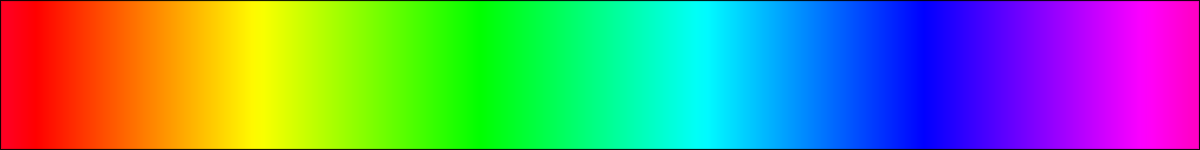
\includegraphics[width = 4.25cm, height = .3cm]{\here/colorbars/rb.png}};


\node[draw = black, thick, inner sep = 0pt, anchor = north] (cb4) at (group1 c2r1.south){
\includegraphics[width = 4.25cm, height = .3cm]{\here/colorbars/cividis.png}};
\node[draw = black, thick, inner sep = 0pt, anchor = north] (cb5) at (cb4.south){
\includegraphics[width = 4.25cm, height = .3cm]{\here/colorbars/batlow.png}};
\node[draw = black, thick, inner sep = 0pt, anchor = north] (cb6) at (cb5.south){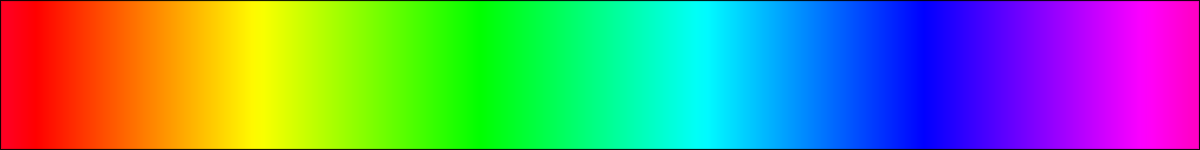
\includegraphics[width = 4.25cm, height = .3cm]{\here/colorbars/rb.png}};


\node[draw = black, thick, inner sep = 0pt, anchor = north] (cb7) at (group1 c3r1.south){
\includegraphics[width = 4.25cm, height = .3cm]{\here/colorbars/cividis.png}};
\node[draw = black, thick, inner sep = 0pt, anchor = north] (cb8) at (cb7.south){
\includegraphics[width = 4.25cm, height = .3cm]{\here/colorbars/batlow.png}};
\node[draw = black, thick, inner sep = 0pt, anchor = north] (cb9) at (cb8.south){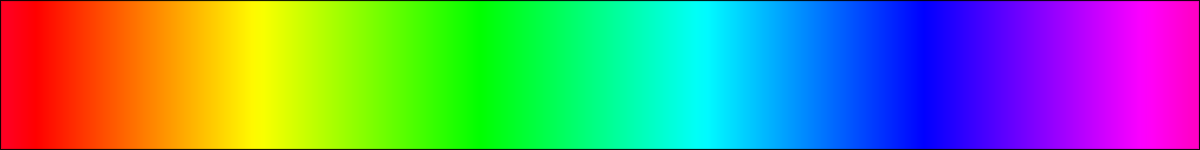
\includegraphics[width = 4.25cm, height = .3cm]{\here/colorbars/rb.png}};

\begin{groupplot}[
		group style = {
			group size = 3 by 1,
			vertical sep = .25cm,
			horizontal sep = .1cm, 
			},
		width = 4.25cm,
		height = 4cm,
		enlargelimits = 0.05,
		simpleax1,
		% ytick = {0,50},
		xticklabel = \empty,
		% xmin = 0.5,
		% xmax = 10.5,
		ymin = 0,
		ymax = 5.5,
		ytick pos = right, 
		yticklabel pos = right,
		scale only axis,
		enlargelimits = false,
		% xtick = {1.5,...,10.5},
		legend style = {
			at = {(0.5,1)},
			anchor = south,
			legend1},
		legend columns = 3,
		xtick = \empty,
		]


		\nextgroupplot[ymax = 100, ylabel = \empty, yticklabel = \empty]
		\addplot[ultra thick, hcqred]table[]{cmap_analytics/rb_L.txt};

		\nextgroupplot[xshift = .9cm, ylabel = \empty, yticklabel = \empty]
		\addplot[ultra thick, hcqred]table[y index = 1]{cmap_analytics/rb_d.txt};
		
		% \addlegendentry{$\Delta E^*_{ab}$}
		% \addlegendentry{$\Delta E^*_{2000}$}
		% \addlegendimage{hcqblue, ultra thick, mark = triangle*, mark options = {thin, fill = hcqblue, draw = black}};
		% \addlegendentry{$L$};
		

		\nextgroupplot[ylabel = \empty, yticklabel = \empty, ymax = 100, ytick pos = right, yticklabel pos = right]
		\addplot[hcqred, ultra thick]table[]{cmap_analytics/rb_d_cum.txt};
		% \addplot+[hcqred, ultra thick, mark options = {thin, fill = hcqred, draw = black}]table[y index = 2]{coldiff2000.txt};

		% \addlegendentry{$\Delta E^*_{ab}$}
		% \addlegendentry{$\Delta E^*_{2000}$}
		% \addlegendimage{hcqblue, ultra thick, mark = triangle*, mark options = {thin, fill = hcqblue, draw = black}};
		% \addlegendentry{$L$};


		% \nextgroupplot[]
		% \addplot+[hcqyellow, ultra thick, mark options = {thin, fill = hcqyellow, draw = black}]table[y index = 3]{coldiffLab.txt};
		% \addplot+[hcqred, ultra thick, mark options = {thin, fill = hcqred, draw = black}]table[y index = 3]{coldiff2000.txt};


		% \addlegendentry{$\Delta E^*_{ab}$}
		% \addlegendentry{$\Delta E^*_{2000}$}
		% \addlegendimage{hcqblue, ultra thick, mark = triangle*, mark options = {thin, fill = hcqblue, draw = black}};
		% \addlegendentry{$L$};

	\end{groupplot}

	\node[text width=1em, anchor=west]at(group1 c1r1.north west){\subcaptionbox{\label{cmA}}{}};
	\node[text width=1em, anchor=west]at(group1 c2r1.north west){\subcaptionbox{\label{cmB}}{}};
	\node[text width=1em, anchor=west]at(group1 c3r1.north west){\subcaptionbox{\label{cmC}}{}};
\end{tikzpicture}

	\caption{Note: Scales are not directly comparable! But shape of each individual line is what matters here.}
	\label{fig:cmapanalytics}
\end{figure}


Here is how you define a new ColorScheme:
\begin{listing}[h]
\begin{minted}[xleftmargin = 1.5cm]{julia} 
using Colors, ColorSchemes
cividis_cols = ColorSchemes.cividis.colors
cividis_protanopic = ColorScheme(protanopic.(cividis_cols, 1))
\end{minted}
\end{listing}

